
\section{Introduction}\label{sec:intro}

\paragraph{What is new.}
% gloss: labeled Markov chain
% gloss: feasible
% gloss: held test
% gloss: word test
% gloss: P-complete
% gloss: PSPACE-hard
% gloss: fine reachability
\begin{itemize}
\item \emph{A sharp complexity boundary} (Theorem~\ref{thm:boundary}).
% gloss: configuration (defined in Section 1.1, as the block's last sentence says)
% gloss: profile
% gloss: at a fixed profile
% gloss: word test
For labeled Markov chains with held tests: can two feasible configurations
at a fixed profile be joined by arbitrarily small feasible rational steps?
% gloss: P-complete
% gloss: PSPACE-hard
This is P-complete when every word test compares single words, and
PSPACE-hard when exactly one compares a word with the sum over two distinct
words and the rest compare single words.
% gloss: signed core
\item \emph{The signed core} (Theorems~\ref{thm:core}
and~\ref{thm:fixed-profile}), a combinatorial invariant that decides the
tractable side, with short certificates for both answers.
% gloss: budgeted signed-binomial system
\item \emph{A model-free version} (Corollary~\ref{cor:intro-algebraic}).
For budgeted signed binomials with a promised bounded rational solution
set, rational fine connectivity is P-complete. Allowing a growing number
of equations $x_j+y_j=1$ makes it PSPACE-hard.
% gloss: acquisition timing
\item \emph{Timing matters} (Theorem~\ref{thm:acquisition}). Adding a test
early can block revisions that adding it late allows.
\end{itemize}
Section~\ref{sec:question} defines the terms, and
Theorem~\ref{thm:intro-boundary} and Table~\ref{tab:results} give the
precise statements.


\subsection{The question}\label{sec:question}

Reconfiguration problems ask whether one feasible solution of a
constraint system can be turned into another by small steps that each
stay feasible~\cite{gopalan,hearndemaine,ito}.
% gloss: feasible
We ask this question for rational parameters in a family of Markov chains whose
transitions carry labels~\cite[Definition~1]{chenkiefer2014}.
% gloss: labeled Markov chain
A \defterm{word test} compares \defterm{words}, strings of transition
labels, all of the same positive length within the model's length bound.
In a word-against-word test, the joint probability of the first word
and each final observed base state must equal that of the second word,
from every initial state of the chain.
In a \defterm{word-against-pair} test, the single word's joint probability
must equal the sum of the corresponding joint probabilities for two distinct
words. Given two feasible rational parameter vectors at a common profile
(defined below),
% gloss: profile
can one be revised into the other, for every $\varepsilon>0$, by a finite
sequence of feasible rational parameter vectors at that profile? Each step
must change every full-state labeled transition probability by less
than~$\varepsilon$.

The chain is built so that word tests yield simple equations. A
\defterm{full state} $(g,r)$ pairs an observed base state~$g$ with a hidden
\defterm{register} value~$r$. Each label~$m$ moves base states by a
kernel~$Q_m$, and all these kernels share a fixed family of $\pm1$-valued
\defterm{probes} on the base states as eigenvectors. The \defterm{eigenvalue}
$\alpha_{mi}$ of $Q_m$ on probe~$i$ is the label's \defterm{signed bias}:
from any full state, conditional on label~$m$, probe~$i$ keeps its sign with
probability $(1+\alpha_{mi})/2$, and an eigenvalue of zero makes the new sign
fair. On each probe, a word's eigenvalue is the product of its labels'
eigenvalues. A word-against-word test therefore gives binomial equations: one
equating word probabilities, and one \defterm{probe equation} per probe
equating eigenvalue products.

The \defterm{Markov law} of the title is the parameter vector: label
probabilities, eigenvalues, and register tables. A \defterm{configuration}
pairs a parameter vector with its \defterm{profile}: positive labeled
transitions, register groupings at each level (Section~\ref{sec:problem}),
and \defterm{held} tests.
% gloss: held test
We keep this profile fixed; every configuration in the sequence must satisfy
all tests held at its profile.

\begin{figure}[t]
  \centering
  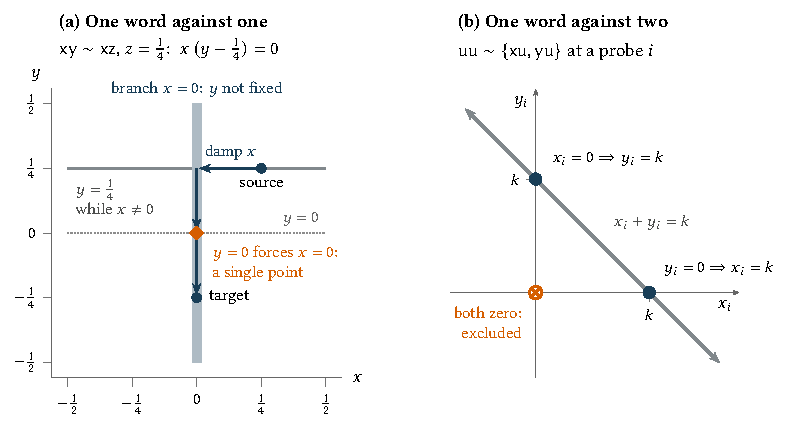
\includegraphics{figures/fig1-mechanism.pdf}
  \Description{Two panels. Panel (a), titled one word against one, plots y against x for the equation x(y - 1/4) = 0 with z = 1/4. A horizontal line at y = 1/4 holds while x is nonzero. On the shaded branch at x = 0, the equation no longer fixes y, and the branch extends from y = -1/2 to y = 1/2. A horizontal arrow damps x from the source (1/4, 1/4) to (0, 1/4). Two downward arrows lead through (0, 0) to the target (0, -1/4). A marked point at the origin notes that setting y = 0 instead forces x = 0, a single point. Panel (b), titled one word against two, shows the load line x_i + y_i = k in the (x_i, y_i) plane at a probe i. Its intercepts at (0, k) and (k, 0) are marked: if one summand is zero the other equals k. The origin is crossed out because both summands cannot vanish.}
  \caption{How the two test syntaxes differ; here $x,y,z$ and $x_i,y_i$ are label eigenvalues on shared $\pm1$ probes (Section~\ref{sec:question}).
% gloss: peeling step (the staged example, next paragraph; the float is placed early for layout)
% gloss: value test (a held value test that fixes one eigenvalue: a calibration)
(a) In the staged example, a held value test fixes (calibrates) $z=1/4$, and the word-against-word test $\mathsf{xy}\sim\mathsf{xz}$ gives $xy=xz$. While $x\neq0$ this fixes $y=1/4$. A \emph{peeling step} damps $x$ to~$0$. On $x=0$ both monomials vanish, so the test still passes while $xy=xz$ stops constraining $y$, letting $y$ move through rationals to $-1/4$. Setting $y=0$ instead forces $x=0$, a single point. (b) In the hard construction of Section~\ref{sec:hard} (with different labels),
% gloss: load label (the calibrated label whose word is compared with the pair; Section 5.1)
one word-against-pair test, with forced label probabilities and a fixed (calibrated) load label, gives the load equation $x_i+y_i=k>0$ at each probe~$i$. If one summand is zero, the other equals~$k$; both cannot vanish. The remaining constraints (Figure~\ref{fig:ncl}) decide which points on this line and which moves are feasible, and at a given feasible configuration an edge may allow only one orientation. In both panels only eigenvalues vanish; the set of positive labeled transitions does not change.}\label{fig:mechanism}
\end{figure}

Two small examples, each with two base states and one probe, show what is at
stake: the \defterm{staged example} (displayed labels $\mathsf x,\mathsf y,\mathsf z$;
Figure~\ref{fig:mechanism}(a)) and the \defterm{sign example} (labels
$\mathsf y,\mathsf z$). Throughout, each italic letter $x,y,z$ denotes the
eigenvalue of the matching roman label. In both examples, a held
\defterm{calibration} fixes $z=1/4$. In the staged example, the held word
test $\mathsf{xy}\sim\mathsf{xz}$ gives $xy=xz$, fixing $y=1/4$ while
$x\neq0$. A \defterm{peeling step} multiplies each eigenvalue by $t^{\eta}$,
with its own nonnegative integer weight~$\eta$, as $t$ falls from $1$ to~$0$.
The weights must preserve every binomial equation \defterm{active} on the
starting support. An equation is active there exactly when neither monomial
is forced to vanish by zeros outside that support. Here
$\eta_x=1$ and $\eta_y=\eta_z=0$, sending $x$ to~$0$. The word test still
passes, its probe equation becomes inactive, and $y$ then moves to $-1/4$ in
arbitrarily fine rational steps.

The sign example has a one-value register and a probability floor of $1/2$, a
lower bound on each label's probability;
% gloss: probability floor
since the two label probabilities sum to~$1$, both equal $1/2$. With the
calibration $z=1/4$ and $\mathsf{yy}\sim\mathsf{zz}$ held, the only feasible
values of $y$ are $1/4$ and $-1/4$. Switching signs changes each labeled
transition-table entry for $\mathsf y$ by $1/8$ in absolute value and fixes
the $\mathsf z$ entries, so a feasible sequence joins them exactly when
$\varepsilon>1/8$. Passing the same tests does not settle reachability. We
ask how hard it is to decide \defterm{fine reachability}, the existence of a
feasible connecting sequence at every positive tolerance. We also ask how the
complexity changes when exactly one word test is word-against-pair and all
other word tests compare single words (Figure~\ref{fig:mechanism}(b)).


\subsection{Our results}\label{sec:results-intro}

Our main theorem gives a tractable--hard boundary for reconfiguration of
exact rational parameter spaces. The two-way classification of Gopalan
et al.~\cite{gopalan}, with Schwerdtfeger's
correction~\cite{schwerdtfeger}, and the three-way classification of Kimura and
Suzuki~\cite{kimurasuzuki} are analogies for this change in complexity at
one step of test syntax.
The title's \defterm{one word against two} names the two test syntaxes:
every word test compares one word with one (the \emph{single-word class}),
or exactly one compares a word with two distinct words and the rest compare
single words.
% gloss: value test
Value tests, which fix an eigenvalue or a probability ratio, are allowed in
both classes. The word-against-pair test imposes $1+|I|$ equations
(Section~\ref{sec:problem}), possibly dependent: one mass equation on word
probabilities and one per probe in the probe set~$I$.
Theorem~\ref{thm:intro-boundary} concerns the shared-probe family of
Section~\ref{sec:model}: labeled Markov chains whose labels act by eigenvalues
on shared probes, with a hidden register. Keeping the profile fixed ensures
that hardness does not come from profile changes.

\begin{theorem}[Informal; see Theorem~\ref{thm:boundary}]\label{thm:intro-boundary}
For explicitly presented shared-probe models encoded in binary, given two
rational configurations $A,B$ promised feasible at a fixed profile:
\begin{enumerate}
% gloss: P-complete
\item[(i)] If every word test compares one word with one, fine reachability
is P-complete under deterministic log-space many-one reductions, with
polynomial-size, polynomial-time-checkable certificates for both answers.
\item[(ii)] If exactly one word test compares a single word with the sum over
two distinct words and all others compare single words, fine reachability is
PSPACE-hard under polynomial-time many-one reductions. The same reduction
proves PSPACE-hardness of sequence existence at a supplied positive rational
tolerance whose reciprocal is polynomially bounded in the length of the
reduction's input.
\end{enumerate}
\end{theorem}

% gloss: signed core
% gloss: G9
% gloss: finely reachable (Section 1.1, fine reachability)
% gloss: reversal (Section 2.1)
\paragraph{Part (i) in words.} In the single-word class, $B$ is finely
reachable from $A$ exactly when both have the same signed core under the
profile's eigenvalue constraints, including the fixed reversal equations
(Theorem~\ref{thm:fixed-profile}; omitting reversal equations can change the
verdict).
The signed core records only the eigenvalue coordinate indices surviving
iterated peeling and their signs, not their magnitudes.
Certificates record peeling stages and a terminal Gordan certificate for each
endpoint, containing no connecting sequence. %
There are algebraic instances for which every feasible connecting sequence
at tolerance $1/4$ contains a coordinate value whose reduced denominator has
exponentially many binary digits in the number of coordinates
(Proposition~\ref{prop:long-sequences}).

\paragraph{Part (ii) in words.} The reduction is from nondeterministic
constraint logic (NCL)~\cite{hearndemaine}. Each edge becomes a probe whose
nonzero summands in the load equation $x_i+y_i=k>0$
(Figure~\ref{fig:mechanism}(b)) give its candidate orientations. A zero
summand forces the other to equal~$k$, though both may be nonzero in between.

% gloss: cover
% gloss: profile step
% gloss: attained (Section 2.3)
\paragraph{The strengthening.} Theorem~\ref{thm:directed} also allows
profile steps to a covering attained profile (adding tests, shrinking
support, or refining register partitions; Section~\ref{sec:directed}) while
keeping label probabilities and eigenvalues, and register tables when support
is unchanged. In the single-word class, fine reachability holds exactly when
the target profile is at or above the source profile and both signed cores
agree under the source profile's constraints.

\paragraph{Scope.} Both lower bounds hold with every test held throughout
and a one-value hidden register; Theorem~\ref{thm:boundary} lists the
remaining restrictions.
% gloss: exactly one word-against-pair test
% gloss: G5
``Exactly one'' counts word-against-pair tests in the model's word-test list;
other word tests and calibrations are unlimited. We prove no upper bound for
part~(ii); one in PSPACE would put rational-zero existence for integer
polynomials in PSPACE (Theorem~\ref{thm:rational-roots}).

\begin{corollary}[The model-free form, informal; see Corollaries~\ref{cor:algebraic} and~\ref{cor:real-complexity}]\label{cor:intro-algebraic}
For an explicit binary budgeted signed-binomial system (equations
$x^a=c\,x^b$ with $a,b\in\NN^J$ and $c\in\QQ$ on coordinates allowed to be
zero or negative, with $\ell^1$ budgets)
% gloss: ℓ¹ budget κ (absolute-value budgets; Section 2.1)
and two supplied feasible rational points:
\begin{enumerate}
\item[(i)] Under the promise that the feasible rational set is bounded,
\defterm{fine connectivity} (joining them at every rational $\varepsilon>0$
by feasible rational steps changing each coordinate by less than~$\varepsilon$)
is P-complete under deterministic log-space many-one reductions meeting the
promise.
% gloss: affine trinomial
\item[(ii)] Allowing a growing number of scalar affine trinomials
$x_j+y_j=k$ (even with $k=1$ throughout) makes fine connectivity PSPACE-hard
under polynomial-time many-one reductions meeting the same promise, with no
upper bound proved here.
\item[(iii)] In the full real locus, membership of two feasible rational
points in one real path component is P-complete for budgeted binomial
systems, and PSPACE-complete with a growing number of equations $x_j+y_j=1$
(Corollary~\ref{cor:real-complexity}); neither upper bound requires
boundedness.
\end{enumerate}
\end{corollary}

\paragraph{Reading the corollary.} The split already occurs for explicit
algebraic systems, with no Markov model. The tractable side contrasts with
real two-point connectivity, which is PSPACE-hard already for noncrossing
planar tree-linkage configuration spaces~\cite[Theorem~2]{altknauerrotewhitesides}.
Following Canny~\cite{canny93}, Basu, Pollack and Roy give a singly
exponential roadmap algorithm for explicit real semialgebraic sets with
algebraically encoded endpoints~\cite[Theorem~3]{basupollackroy}.
The direct algebraic reduction uses $|E|$ normalized affine trinomials
(Section~\ref{sec:real-ncl}), leaving PSPACE-hardness with one scalar affine
trinomial open.

\begin{table}[tp]
\caption{Results at a glance. Decision inputs are explicitly encoded in
binary, with supplied feasible rational endpoints. P-completeness is under
deterministic log-space many-one reductions, and PSPACE lower bounds are
under polynomial-time many-one reductions. Source~$A$, target~$B$; $\preceq$
is the profile order (Section~\ref{sec:directed}); $A^+$ is $A$ after an
acquisition.}\label{tab:results}
\footnotesize\setlength{\tabcolsep}{4pt}\renewcommand{\arraystretch}{0.88}
\begin{tabular}{@{}>{\raggedright\arraybackslash}p{0.25\linewidth}p{0.60\linewidth}p{0.11\linewidth}@{}}
\toprule
Problem & Result & Where\\
\midrule
\multicolumn{3}{@{}l}{\emph{Main results}}\\[2pt]
Single-word class, fixed profile & P-complete, with polynomial-size,
polynomial-time-checkable certificates for both answers; decided by equal
signed cores under the common profile's constraints. &
Thms~\ref{thm:boundary}(i), \ref{thm:fixed-profile}\\
% gloss: G9
Single-word class, with profile steps & P-complete, with the same certificate
guarantees; holds exactly when $p_A\preceq p_B$ and signed cores agree under
the source profile's constraints. & Thm~\ref{thm:directed}\\
% gloss: G5
% gloss: G7
Exactly one word-against-pair test & Fixed profile: PSPACE-hard for fine
reachability and at a supplied tolerance (verdict agrees at that tolerance
and below on NCL outputs); rational-zero existence reduces to it; no upper
bound proved. & Thms~\ref{thm:boundary}(ii), \ref{thm:rational-roots}\\
Budgeted binomials: fine connectivity (bounded rational set) & P-complete. &
Cor.~\ref{cor:algebraic}\\
\quad plus growing affine trinomials $x_j+y_j=k$ (same promise) &
PSPACE-hard; no upper bound proved. & Cor.~\ref{cor:algebraic}\\
Budgeted binomials: real path-component membership & Full real locus, two
supplied feasible rational endpoints: P-complete for budgeted binomials, and
PSPACE-complete with growing equations $x_j+y_j=1$; upper bounds need no
boundedness, and hardness already holds on bounded real loci. &
Cor.~\ref{cor:real-complexity}\\[3pt]
\multicolumn{3}{@{}l}{\emph{Further results}}\\[2pt]
Single-word class, no nonzero calibration held at source & Fine reachability
holds exactly when $p_A\preceq p_B$. & Thm~\ref{thm:no-calibration}\\
% gloss: undecidable
% gloss: G14
One word-against-pair test, fixed counts & For each fixed $N$, quartic
rational solvability reduces to fine reachability and sequence existence at
one fixed positive tolerance. Probe and label counts depend only on~$N$.
Undecidability is conditional on the Bhargava--Burungale quartic
theorem~\cite[Corollary~1.2(3)]{bhargavaburungale}. & Cor.~\ref{cor:quartic}\\
One word-against-pair test, zero probes & If the test is unheld at the
source, the directed profile order decides fine reachability. If held, two
subcases are polynomial-time. The remaining subcase has an exact
rational-ratio closure criterion whose decidability is open. & Props.~\ref{prop:zero-probes},
\ref{prop:zero-probe-closure}\\
Real versus rational, one word-against-pair test & Examples with zero probes
(and a held probability-ratio test) and with one probe have a real path but
fail fine rational reachability. & Props.~\ref{prop:one-probe},
\ref{prop:zero-probe-fermat}\\
One-state subclass & Length-two tests with growing word-against-pair tests:
PSPACE-hard at a fixed profile and at the supplied tolerance; rational-zero
existence also reduces to it. & Prop.~\ref{prop:one-state}\\
Acquisition timing (test acquired before or after revision) & Early
acquisition can block fine reachability that late acquisition allows, even when
both endpoints pass the new test. For the feasible acquisition keeping the
parameter vector fixed, with $p_A\preceq p_{A^+}\preceq p_B$, two signed-core
checks decide timing in polynomial time (single-word class). With both
word-test shapes, the criterion compares components in the projected rational
closures $\mathcal K_{p_A}$ and $\mathcal K_{p_{A^+}}$ (no general algorithm
given). & Thms~\ref{thm:acquisition}, \ref{thm:projected-components}\\
% gloss: real component
% gloss: G22
Budgeted binomials: real components (no boundedness assumed) & Connected and
path components are classified by the signed core. & Cor.~\ref{cor:real}\\
Separation cutoff for distinct signed cores (bounded rational locus) & Sup
distance $\ge 2^{-D}$, with $\log D$ polynomially bounded in binary system
length excluding endpoints; transfers to the Markov metric. Expanded rational
cutoff denominators can need exponentially many digits. Doubly exponential
scale and repeated-squaring witness via Jeronimo, Perrucci and
Tsigaridas~\cite{jeronimoperruccitsigaridas}. & Prop.~\ref{prop:separation}\\
\bottomrule
\end{tabular}
\end{table}

\paragraph{Contributions.}
\begin{enumerate}
\item \emph{The boundary} (Theorem~\ref{thm:intro-boundary},
Table~\ref{tab:results}). At a fixed profile on promised-feasible rational
inputs, fine reachability is P-complete with polynomial-size certificates for
% gloss: polynomial-size certificates (no connecting sequence; Part (i) in words)
both answers in the single-word class, and PSPACE-hard with exactly one
word-against-pair test.
% gloss: G25
Since the reductions land inside the promise, the single-word problem is in
log-space-uniform NC only if P equals log-space-uniform NC.
To our knowledge, this PSPACE lower bound for fine rational reachability with
exactly one word-against-pair test in this model has not appeared in the
literature. For continuous Petri nets, Fraca and Haddad's Algorithm~2 and
Propositions~27 and~32~\cite{fracahaddad} give the precedents for the
iterated linear-programming upper bound of part~(i) and its lower bound from
monotone circuit value~\cite{goldschlager,greenlawhooverruzzo}.
Here the signed core gives certificates for both answers, and the circuit
reduction uses endpoints sharing a profile and differing in one sign.
\item \emph{The model-free form} (Corollary~\ref{cor:intro-algebraic}). Over
$\RR$, the signed core classifies the components of budgeted signed-binomial
systems without assuming boundedness. For feasible rational endpoints, real
path connectivity agrees with rational fine connectivity when the rational
feasible set is bounded (Corollary~\ref{cor:real}). Real path-component
membership is P-complete, and PSPACE-complete with a growing number of
equations $x_j+y_j=1$ (Corollary~\ref{cor:real-complexity}). The PSPACE
upper bound uses the component algorithm of Heintz, Roy and
Solern\'o~\cite{heintzroysolerno1994components}. We have
not found the rational PSPACE lower bound of
Corollary~\ref{cor:intro-algebraic}(ii) in the literature.
\item \emph{The engine} (Theorems~\ref{thm:core}, \ref{thm:fixed-profile},
\ref{thm:directed} and~\ref{thm:no-calibration}). We have not found
the signed-core classification of Theorem~\ref{thm:core} for bounded
rational feasible sets of budgeted signed-binomial systems stated in the
literature. Newman~\cite{newman}
supplies the confluence antecedent, Tevelev~\cite{tevelev} a chart-limit
antecedent, and \emph{Toric Cubes}~\cite{toriccubes} related fixed-support
geometry. Geiger--Meek--Sturmfels~\cite{geigermeeksturmfels} and
Rauh--Kahle--Ay~\cite{rauhkahleay} give facial-support criteria for positive
model families, while Payne~\cite{payne} and
Soprunova--Sottile~\cite{soprunovasottile} study real toric varieties.
Diaconis--Eisenbud--Sturmfels~\cite{diaconiseisenbudsturmfels} and
Kahle--Rauh--Sullivant~\cite{kahlerauhsullivant} relate discrete
connectivity to binomial ideals for fixed move sets. Our additional steps are
restriction across recomputed supports, the least support, and exact rational
realization under budgets.
\item \emph{Acquisition timing} (Theorems~\ref{thm:acquisition}
and~\ref{thm:projected-components}). Barrett and
Weld~\cite[Sections~3.2--3.3]{barrettweld} study which subgoals can be
achieved and protected in order. Hauser and Latombe analyze component
obstructions at mode intersections~\cite{hauserlatombe}, and Hu, Iyer and
Christensen connect within-manifold roadmaps at
intersections~\cite{huiyerchristensen}. We have not found this
before-and-after criterion for projected rational closures in this model in
the literature.
% gloss: undecidable
% gloss: G14
\item \emph{Exactness} (Corollary~\ref{cor:quartic},
Section~\ref{sec:exactness}). Table~\ref{tab:results} lists the fixed-count
quartic reduction, the real-versus-rational separations, and the zero-probe
cases. That reduction gives undecidability of both target decision problems
for some fixed counts if the Bhargava--Burungale quartic
theorem~\cite[Corollary~1.2(3)]{bhargavaburungale} holds.
\end{enumerate}

\subsection{Techniques}\label{sec:techniques}

The tractable side has one delicate point: tests become inactive as
coordinates vanish. In the staged example, the branch $x=0$ joins opposite
signs of~$y$, so active tests must be recomputed after each peeling step.
Keeping the initial weight balances instead rejects that example
(Figure~\ref{fig:peeling}). Under a fixed test list, permitted peeling steps
restrict to smaller supports, so from a given signed support every terminal
peeling sequence gives the same signed core (Lemma~\ref{lem:restriction}).
After peeling, exact rational interpolation under tight budgets joins points
with the same signed support (Lemma~\ref{lem:interpolation}); in the
P-hardness reduction the surviving signed core computes the circuit.

On the hard side, a positive-sum test keeps constraining when a summand
vanishes: in the load equation $x_i+y_i=k>0$ (Lemma~\ref{lem:engine}) a zero
summand forces the other to carry the load.
A nonzero summand makes the corresponding edge orientation available, and
further tests and budgets encode legality of every represented orientation.
We do not claim that these extra tests and budgets are needed for hardness.
Transfer must hold in both directions and for every feasible step below the
supplied cutoff, including multi-coordinate steps (Section~\ref{sec:transfer}).
The cited hardness results concern different solution spaces or step rules.
Bürgisser and Cucker's Proposition~8.15~\cite{burgissercucker} proves
PSPACE-hardness of deciding whether some point of each of two specified loci lies in one connected
component of the real zero set of one integer polynomial. Their Lemma~8.14
supplies the single-equation construction, and their Remark~8.16 retains
hardness for compact one-dimensional real algebraic sets. The related
results of Cardinal et al.~\cite{cardinal} concern discrete configurations.
Specifically, Cardinal et al.~\cite[Theorem~3.3]{cardinal} prove strong
PSPACE-completeness for subset-sum reconfiguration with 3-moves, and their
Theorem~4.7 proves PSPACE-completeness for single-bit moves with a constant
number of inequalities.

\subsection{Related work}\label{sec:related}

\emph{Reconfiguration.} Gopalan et al.~\cite{gopalan}, with Schwerdtfeger's
correction~\cite{schwerdtfeger}, classify two-solution connectivity for
constraint languages with constants and repeated variables. Ito et
al.~\cite[Section~1]{ito} give the general framework (hard cases in
Theorems~1--2; tractable ones in Theorem~3 and Proposition~2). Cardinal et
al.~\cite{cardinal} and Kimura and Suzuki~\cite{kimurasuzuki} find thresholds
for subset sums and integer linear systems. Hirahara and
Ohsaka~\cite{hiraharaohsaka} and Guruswami et al.~\cite{guruswami} study
approximate reconfiguration, where intermediate assignments may violate a
fraction of constraints. At a fixed profile and tolerance, our problem has
Ito et al.'s adjacency-graph form. However, solutions need not have
polynomial length, fine reachability quantifies over all tolerances, and
every step joins exact feasible rational configurations.

\emph{Real-algebraic connectivity.} Related binomial results include toric
cubes~\cite{toriccubes,basugabrielovvorobjov} and toric component
counts~\cite{soprunovasottile}. Fine connectivity is Akin and Wiseman's chain
relation for the identity on feasible rational points with the fixed sup
metric~\cite[Section~3]{akinwiseman}. With one word-against-pair test, real
component membership can give the wrong rational verdict
(Section~\ref{sec:real-rational}).

\emph{Parametric Markov chains, Petri nets and model repair.} Parameter
synthesis partitions a parametric Markov chain's parameter space by
specifications~\cite{jungesetal2019,hutschenreiterbaierklein}, and model
repair adjusts transition probabilities to meet a specification~\cite{ceska}.
Fatmi et al.~\cite{fatmikiefermainparker} ask whether states or distributions
are language-equivalent or probabilistically bisimilar under some or every
transition-probability assignment permitted by a fixed allowed-edge graph.
Robust reachability separates one perturbation scale from all
scales~\cite{asarinbouajjani,bournezgracahainry,blancbournez,blanc}. These
works concern satisfying valuations, equivalence across valuations, or
perturbed dynamics. By contrast, we study connectivity between two supplied
feasible rational parameter vectors through feasible rational ones under the
held exact tests.

\subsection{Origin of the question}\label{sec:origin}

% lint: program begin
The question arose in the Six Birds program, a series of papers on how
stable descriptions of a finite process form and how they can be strictly
extended~\cite[Sections~4.1--4.2]{foundations1}.
% gloss: Six Birds program
% gloss: held test (Section 1.1)
On the program's reading, retaining held tests models revision without
retraction. In this paper the directed order is defined by retaining held
tests, shrinking table support and refining register partitions
(Section~\ref{sec:directed}).
An earlier step of the series revised a Markov chain while each label's
transition kernel on the base states stayed fixed, a case with an exact
criterion of its own. Once those kernels may change too, two feasible
configurations at ordered profiles need no longer be joined at every
positive tolerance. The program asked whether a configuration can acquire a
new held test through feasible revisions, or whether reachability can fail
even when both endpoint configurations are feasible. This paper asks which
pairs are joined, and how hard it is to tell.
% lint: program end

% ---------------------------------------------------------------------------
\subsection{Formal verification and organization}

\paragraph{Formal verification.} Appendix~\ref{app:verification} records the
Lean~\cite{lean4,mathlib} checks of the signed-core criteria and reduction
correspondences, including selected record and size bounds. The LP resource
bounds and complete binary-transduction and running-time analyses are
written proofs.

\paragraph{Organization.} Sections~\ref{sec:problem}--\ref{sec:hard} state
and prove the boundary, Sections~\ref{sec:timing}--\ref{sec:exactness} treat
timing and exactness, and Sections~\ref{sec:discussion}--\ref{sec:open}
give scope, a reading of the results, and open problems.
